\documentclass{article}

\usepackage[final]{style}
\usepackage[utf8]{inputenc} % allow utf-8 input
\usepackage[T1]{fontenc}    % use 8-bit T1 fonts
\usepackage{hyperref}       % hyperlinks
\usepackage{url}            % simple URL typesetting
\usepackage{booktabs}       % professional-quality tables
\usepackage{amsfonts}       % blackboard math symbols
\usepackage{nicefrac}       % compact symbols for 1/2, etc.
\usepackage{microtype}      % microtypography
\usepackage{verbatim}
\usepackage{graphicx}       % for figures
\usepackage{amsmath}
\usepackage{algorithm}
\usepackage{algpseudocode}
\makeatletter
\def\BState{\State\hskip-\ALG@thistlm}
\makeatother

\title{Lecture \#9: Image Resizing and Segmentation}

\author{
  Mason Swofford, Rachel Gardner, Yue Zhang, Shawn Fenerin \\
  Department of Computer Science\\
  Stanford University\\
  Stanford, CA 94305 \\
  \texttt{\{mswoff, rachel0, yzhang16, sfenerin\}@cs.stanford.edu} \\
}

\begin{document}

\maketitle

\section{Introduction}
The devices people use to view images or videos are of different sizes and shapes. The images or videos that are suitable on one device may look not good on other devices. For that reason, image resizing becomes an important problem. The intuitive idea is to rescale or crop the original image to fit the new device, but that often causes artifacts or even loss of important content in images. This lecture is about how to resize images to preserve important content and limit artifacts.
\subsection{Problem Statement}
Input an image of size $n\times m$ and return an image of desired size $n'\times m'$ which will be a good representative of original image. The expectations are:
\begin{enumerate}
\item The new image should adhere to device geometric constraints.
\item The new image should preserve the important content and structures.
\item The new image should have limited artifacts.
\end{enumerate}
\subsection{Importance Measures}
\begin{enumerate}
\item A function, $S: p \rightarrow [0,1]$, is used to determine which parts in an image are important, then some operators can be used to help change the image. One idea is to use optimal cropping window to find out the most important contents, but this idea may cause loss of important contents.
\begin{figure}[H]
\centering
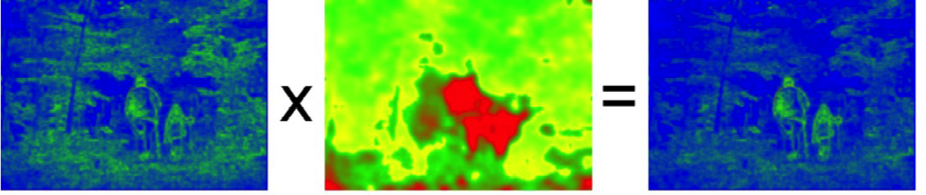
\includegraphics[width=8cm]{Function.png}
\caption{Importance Measurement by function method. Source: Lecture 7-11.}
\end{figure}
\item There are also more sophisticated measurements such as using attention models, eye tracking (gaze studies), face detectors, etc.
\begin{figure}[H]
\centering
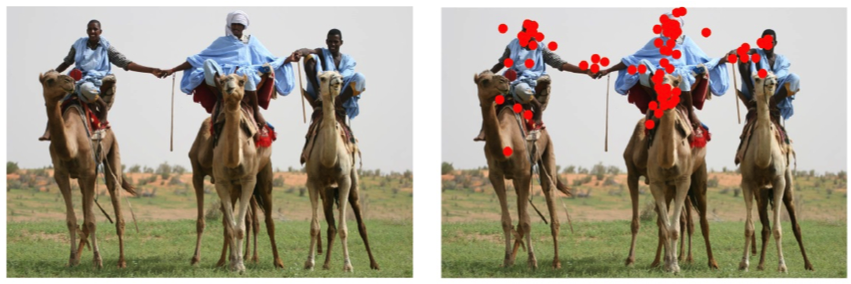
\includegraphics[width=8cm]{Tracking.png}
\caption{Importance Measurement by more sophisticated method. Source: Lecture 7-11, \textit{Judd et al. ICCV09 Learning to predict where people look.}}
\end{figure}
\end{enumerate}

% Lecture 7 - 20 to 40
% Yue
% Gustavo 40 to 60
\section{Seam Carving}
\subsection{Basic Idea}
Intuitively, human vision is more sensitive to edges. Thus a simple but effective idea is to try to remove contents from smoother areas and preserve those more informative edges using the gradient-based energy function. It is defined as
$$
E(I) = |\frac{\partial}{\partial x}I| + |\frac{\partial}{\partial y}I|
$$
Unimportant contents should be pixels with smaller values of energy function.
\subsection{Pixel Removal}
Different ways to remove unimportant pixels can lead to different results. From the figures below, the first two methods mess up the image. The last one works much better but causes plenty of artifacts in the new image.
\begin{enumerate}
\item Removing all pixels with less energy.
\item Removing the rows of pixels with least-energy.
\item Removing the columns of pixels with least-energy.
\end{enumerate}
\begin{figure}[H]
\centering
\hspace*{1.2cm}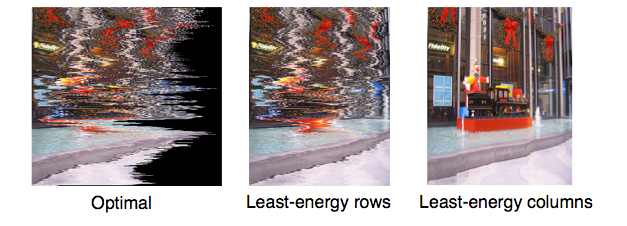
\includegraphics[width=8cm]{Pixel_Removal.png}
\caption{The effects of different pixel removal methods. Source: Lecture 7-18}
\end{figure}
\subsection{A Seam}
\begin{enumerate}
\item A seam is defined as a connected path of pixels from top to bottom (or left to right). For top-to-bottom pixel, we shall pick exactly one pixel from each row. The mathematical definition is
$$
s^x = \{s_i^x\}_{i=1}^n = \{x(i),i\}_{i=1}^n, s.t. \forall i, |x(i) - x(i - 1)| \leq 1
$$
$$
s^y = \{s_j^y\}_{j=1}^m = \{j,y(j)\}_{j=1}^m, s.t. \forall j, |y(j) - y(j - 1)| \leq 1
$$
\item The optimal seam is the seam which minimizes the energy function, based on pixel gradients.
$$
s^{*} = argmin_s E(s), \quad \textrm{where} \quad E(I) = |\frac{\partial}{\partial x}I| + |\frac{\partial}{\partial y}I|
$$
\begin{figure}[H]
\centering
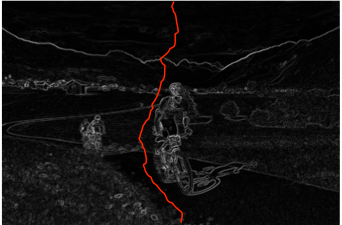
\includegraphics[width=8cm]{Optimal_Seam.png}
\caption{The red line shown in the figure is the optimal seam. Source: Lecture 7-22}
\end{figure}
\item The recursion relation can be used to find the optimal seam. If $M(i,j)$ is defined as the minimal energy cost of a seam going through pixel $(i,j)$, the recursion relation is
$$
M(i,j) = E(i,j) + min(M(i-1,j-1), M(i-1,j), M(i-1,j+1))
$$
This problem can be solved efficiently by using dynamic programming in $O(snm)$, $s=3$ in the original algorithm.
Given the energy function value as
\begin{figure}[H]
\centering
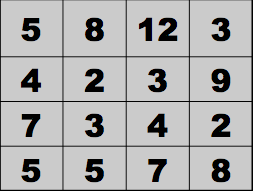
\includegraphics[width=4cm]{energy.png}
\caption{An example of energy function to explain seam carving algorithm. Source: Lecture 7-24}
\end{figure}
The recursion relation gives
\begin{figure}[H]
\centering
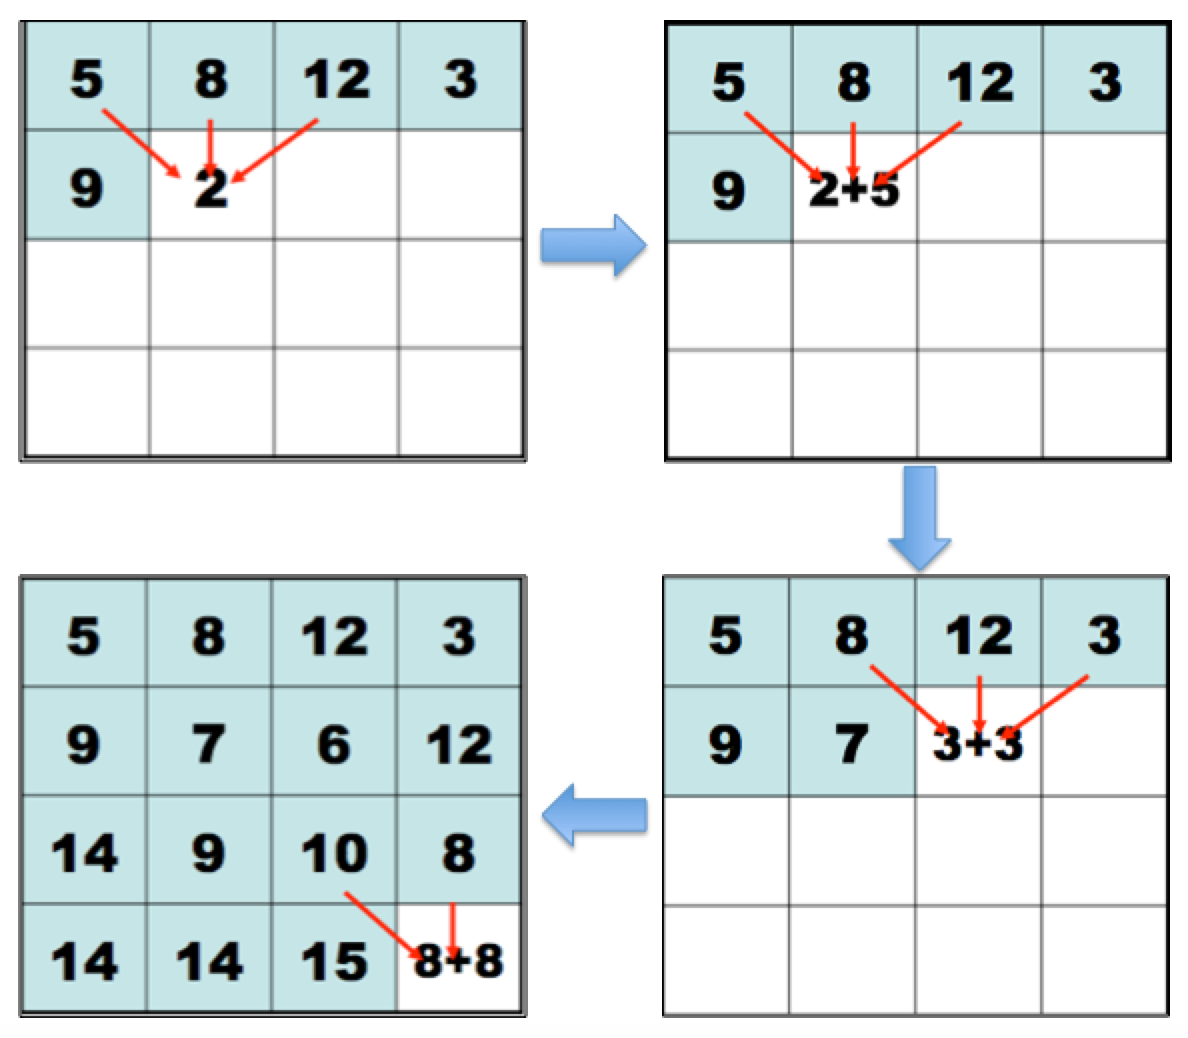
\includegraphics[width=8cm]{findseam1.png}
\caption{Using relation resursion to compute seam cost. Source: Lecture 7-(24-27)}
\end{figure}
\item To search for the optimal seam, backtracking method is introduced. Starting from the pixel at the bottom with the lowest energy function, then goes up until the top. 
\end{enumerate}
\begin{figure}[H]
\centering
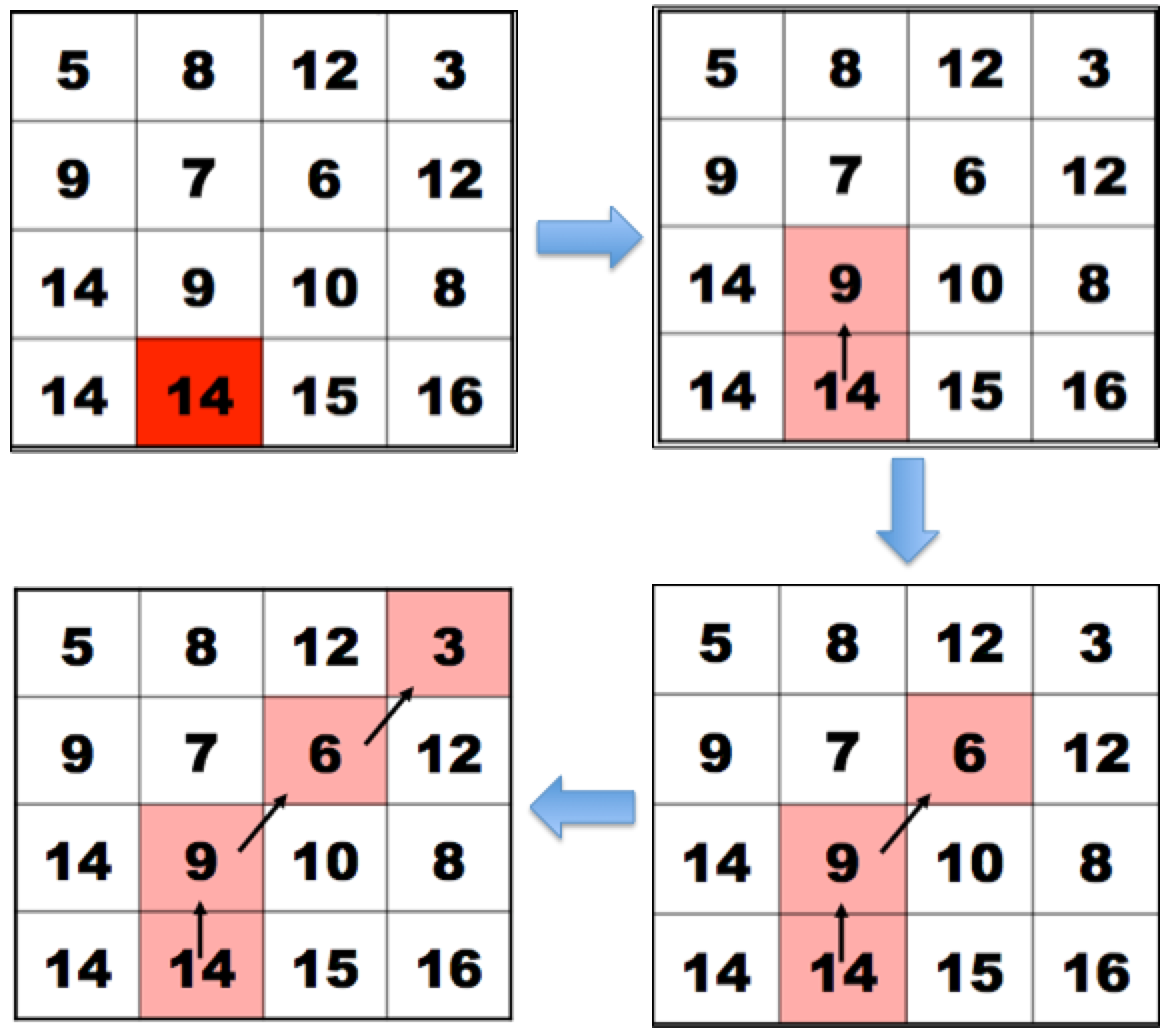
\includegraphics[width=8cm]{backtrack.png}
\caption{Using backtrack to find the optimal seam. Source: Lecture 7-(28-31)}
\end{figure}
\subsection{Seam Carving Algorithms}
This algrithm runs $O((n-n')mn)$. In each loop, each update of $E$, $s$ and $im$ takes $O(mn)$. For vertical resizing, the image could be transposed so that the same algorithm can be used.
\begin{algorithm}
\caption{Seam-Carving}\label{euclid}
\begin{algorithmic}[1]
\State $im \gets \textit{original image of size m $\times$ n}$
\State $n' \gets \textit{desired image size n'}$
\State
\BState \emph{Do (n-n') times}:
\State \hspace{0.5cm} $E \gets \textit{Compute energy map on im}$
\State \hspace{0.5cm} $s \gets \textit{Find optimal seam in E}$
\State \hspace{0.5cm} $im \gets \textit{Remove s from im}$
\State
\BState \emph{return im}
\end{algorithmic}
\end{algorithm}


Average energy of images will increase given that seam carving algorithm removes low energy pixels. With seam carving algorith, aspect ratio, removal of objects, resizing can be accomplished. Result is same if image is flipped. When resizing, we have to remove both horizontal and vertical seams. One can solve the order of adding and removing seams in both directions by dynamic programming. Specifically, the recurrence relation is: $T(r,c)=min(T(r-1,c)+E(s^x(I_{n-r-1\times m-c})),T(r,c-1)+E(s^y(I_{n-r\times m-c-1})))$ for more information refer to the SIGGRAPH paper on seam carving \cite{siggraphseamcarving}. 

\begin{center}
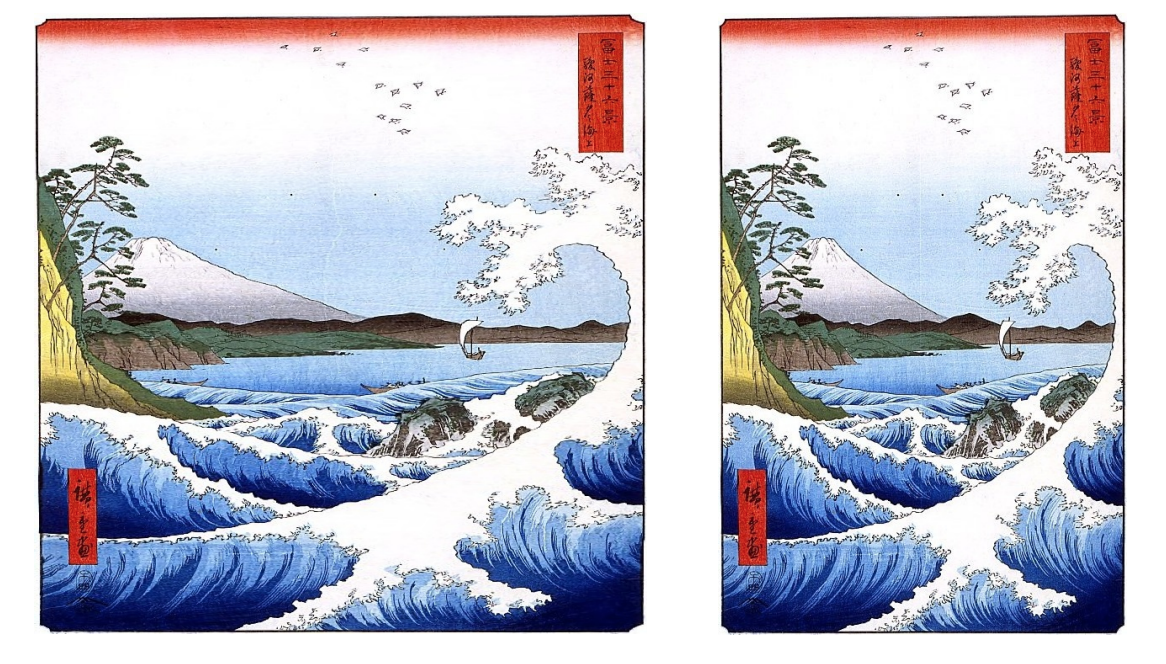
\includegraphics[width=8cm]{content_aware_resizing.png} \\
Figure 8: The Sea off Satta, Hiroshige woodblock print (Public Domain)
\end{center}

% Lecture 7 - 60 to [end]
% Rachel
\section{Advanced Seam Carving}
\subsection{Image Expansion}
We can use a similar approach to increase the size of images. By expanding the least important areas of the image (as indicated by our seams), we can increase the dimensions of the image without impacting the main content. A naive approach would be to simply iteratively find and duplicate the lowest energy seam. However, such a method would result in an image as follows:

\begin{center}
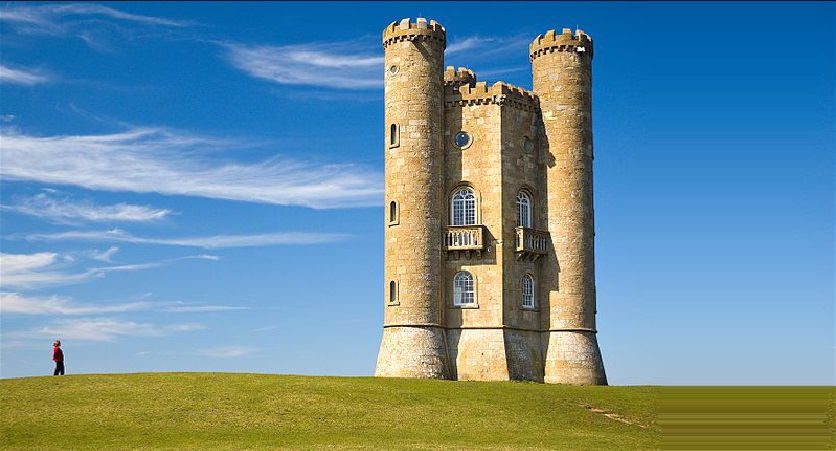
\includegraphics[width=8cm]{Naive_Castle_Resizing.jpg} \\
Figure 9: https://commons.wikimedia.org/wiki/File:Broadway\_tower\_edit.jpg
\end{center}
On the right side of the image, one seam has been duplicated many times over. This is because each time the program goes to find a new seam, it finds the same seam (since that seam is still the one with least energy). A more effective implementation is to find the first $k$ seams at once, then duplicate each of them, as shown:

\begin{center}
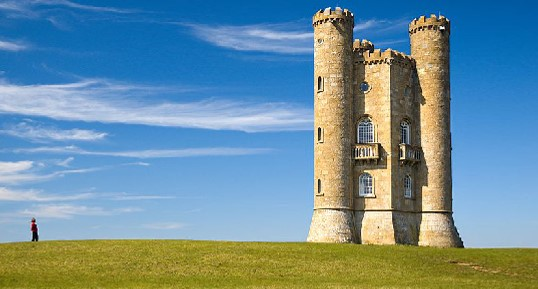
\includegraphics[width=8cm]{Smart_Resizing.jpg} \\
Figure 10: https://commons.wikimedia.org/wiki/File:Broadway\_tower\_edit.jpg
\end{center}
The image above looks much more natural. Note however that this method can only enlarge the image by 2x (since there simply aren't enough seams to duplicate). For very dramatic enlargements, you can instead iteratively enlarge by 1.4-1.5x.

\subsection{Multi-Size Image Representation}
While we've seen that image resizing can be very effective, it is still very compute-intensive. In practice, many images will actually be stored alongside a representation of their seams so as to make them easier to resize. These seam representations are the same dimensions as the image, but instead of pixel intensities, they have numbered paths ordering seams from least to most energy. Note that in order to calculate multiple seams at a time in the pre-processing step, the energy of the image must be recalculated after simulating the removal of each seam. See below for an example of such a representation:
\begin{center}
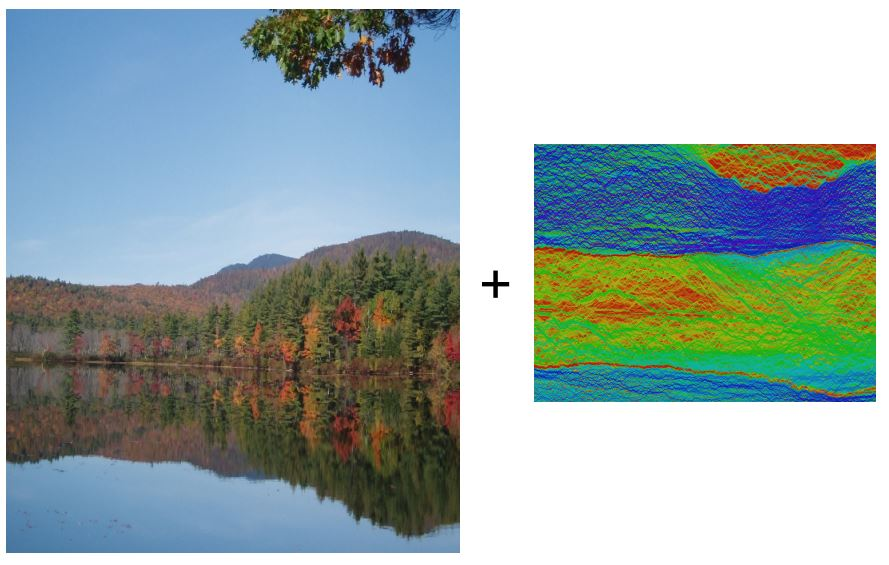
\includegraphics[width=8cm]{resizing_representation.JPG} \\
Figure 11: Dr. Ariel Shamir, SIGGRAPH 2007; CS131 Lecture Slides
\end{center}
Given this representation, a program seeking to remove $k$ seams from the original image can simply remove the pixels corresponding to those labeled 1 through $k$ in the seam image (at right).
\subsection{Object Removal}
By allowing users to specify which areas of the image to give high or low energy, we can use seam carving to specifically preserve or remove certain objects. The algorithm will then choose seams specifically so that they go through the given object (in green below).

\begin{center}
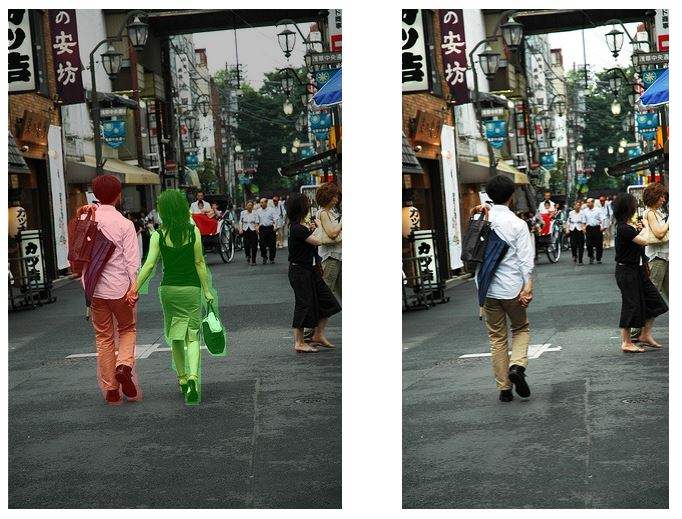
\includegraphics[width=8cm]{object_removal.JPG} \\
Figure 12: Dr. Ariel Shamir, Shai Aiden SIGGRAPH 2007
\end{center}

%Shawn Fenerin
\subsection{Limitations}
As we have seen, seam carving is an extremely capable method of effectively resizing an image. However, there are limitations. The primary limitation is the lower and upper limit to effectiveness as the size of the image is drastically changed.  The second limitation is the failure of seam carving to recognize important features in the context of an object that can be low energy. Let us consider the image below.
\begin{center}
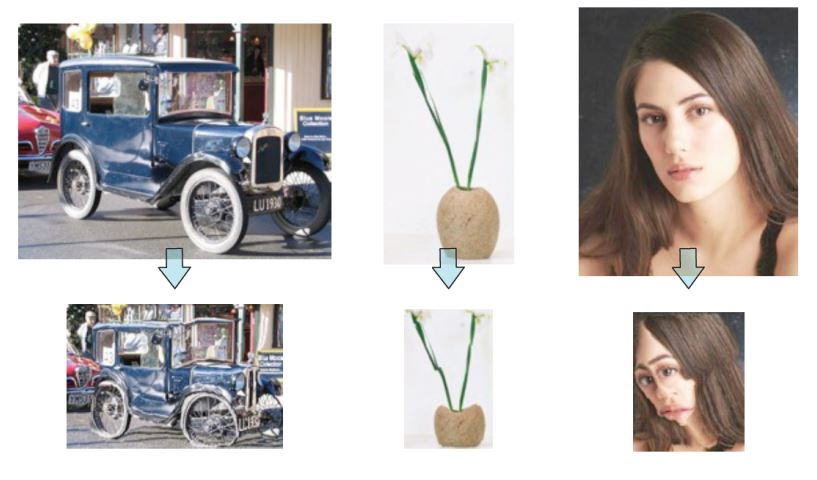
\includegraphics[width=8cm]{seam_carving_limitations.JPG} \\
Figure 13: CS131 Lecture 7, slide 71
\end{center}

We can see that flat, smooth areas with low gradients that are important to the image, like the cheeks and forehead of the women, are being removed as the image is reduced. While they clearly have less energy as far as the algorithm is concerned, they are important features to human perception that should be preserved. To overcome issues like these, we can modify our energies to consider additional information. For example, we could use a face detector or apply user constraints like in the image below. 

\begin{center}
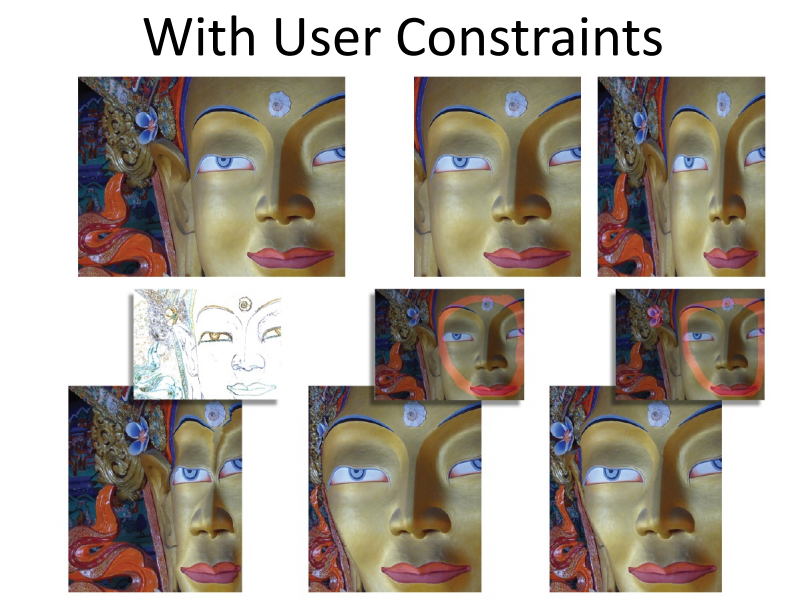
\includegraphics[width=8cm]{user_constraints.PNG} \\
Figure 14: Seam Carving	for	Content-Aware Image	Resizing – Avidan and Shamir	2007
\end{center}
% * <sfenerin@stanford.com> 2017-10-31T02:00:41.390Z:
%
% ^.

\subsection{Forward Energy}
When we seam carve, we are removing the lowest energy pixels and preserving the highest energy pixels. As we do this, the average energy of the image is increased which can lead to artifacts and jagged edges. A way to avoid this issue is to instead focus on removing seams that insert the least energy to the image. In forward energy, our original accumulated cost matrix is modified with adding the forward energy from corresponding new neighbors as seen in the image below. Our previous method can be considered "backward" energy. 

\begin{center}
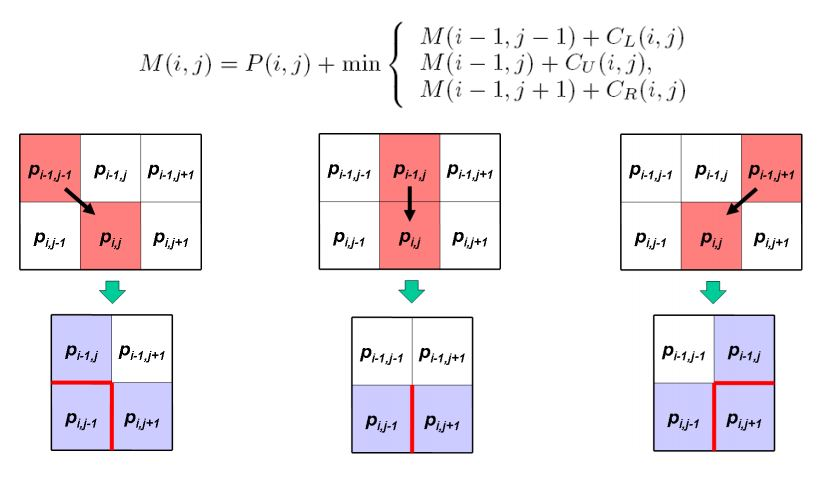
\includegraphics[width=8cm]{forward_energy_calculation.JPG} \\
Figure 15: Lecture 7-71
\end{center}

You can see the benefits of an approach such as this in the following image. With the traditional "backward" energy approach, jagged edges being to appear along the handle of the wrench and the stem of the plant. With the "forward" energy approach, as we are now minimizing added energy, the smoothness of edges is maintained. 

\begin{center}
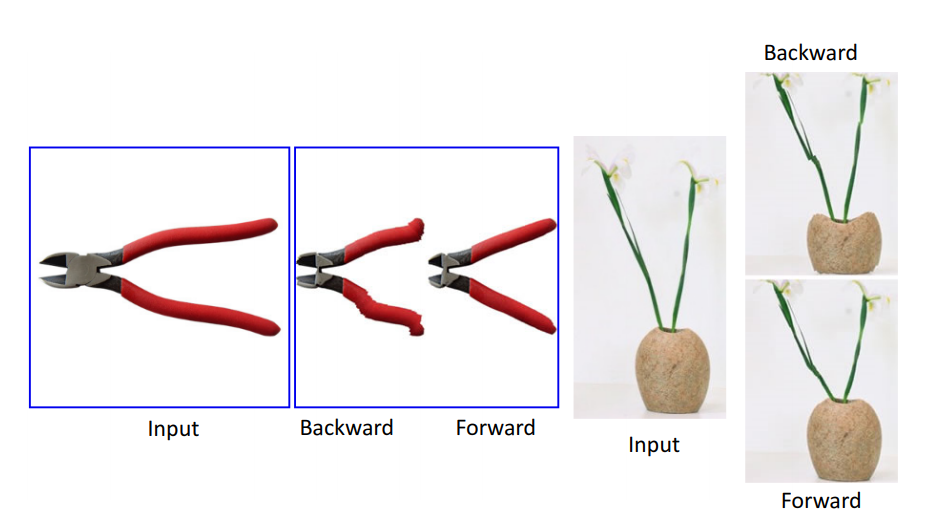
\includegraphics[width=8cm]{forward_energy.PNG} \\
Figure 16: Seam	Carving	for	Content-Aware	Image	Resizing	– Avidan and	Shamir	2007
\end{center}

\subsection{Seam-Carving in Videos}
Since we've shown the powerful capabilities of seam carving, the next question is to consider applying this to video. However, while the seam-carving algorithms with a variety of tweaks can intelligently resize a single image well, it starts to encounter issues with resizing video. It turns out, video is a much more difficult problem. We face two primary issues. 

First, let us consider a single minute of film at 30fps. In that minute, we have 1800 frames. If our seam carving algorithm takes a full minute to process an image, it would take us 30 hours to completely process the video. 

The second issue is with temporal coherency. One can consider the intuitive and naive approach of seam carving frame by frame. However, from frame to frame, there is important context which may not necessarily be preserved. Since the human eye is particularly sensitive to movement, this failure to consider context across images can create a poor looking video with clear distortion from frame to frame. There is no coherency to changes across frames. The less naive approach is to consider the video as a three dimensional space where each vertical plane is an image from the video. From there, you can find the lowest energy 2D seam throughout the whole video. This produces much better results but is still not quite perfect. 
\begin{center}
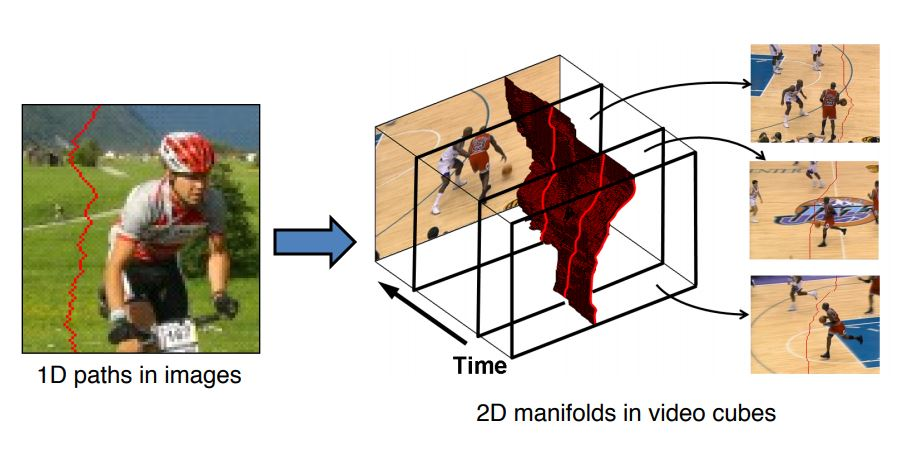
\includegraphics[width=8cm]{video_retargeting.JPG} \\
Figure 17: Improved Seam Carving for Video Retargeting, Rubinstein et al. 2008
\end{center}

This 3D representation gives us the same capabilities as 2D Seam-Carving such as object removal, resizing, etc.
% Lecture 12 - 1 to 20
% Mason
\section{Segmentation}
Sometimes in computer vision we want to identify groups of pixels that go together. We call this image segmentation. Humans naturally perform image segmentation. For instance, two people looking at the same optical illusion might see different things, all depending on how their brain segments the images. For instance, in the image below, you might see zebras, or you might see a lion. 
\begin{center}
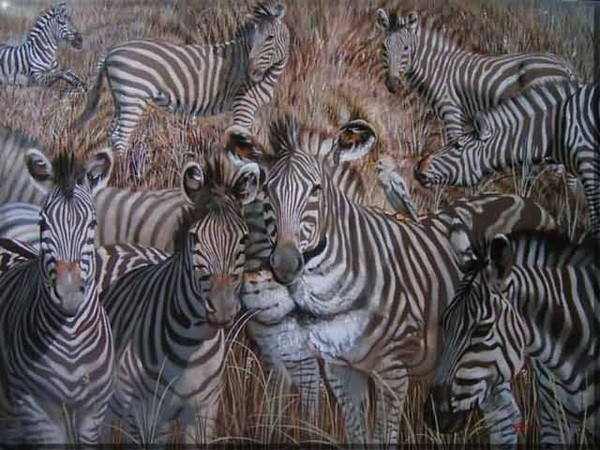
\includegraphics[width=8cm]{lion.jpg} \\
Figure 18: https://www.weirdoptics.com/hidden-lion-visual-optical-illusion
\end{center}

There are many reasons we might want a computer to be able to segment  an image. We might want to separate an image into coherent objects similar to how a human would. Here are two examples of this type of segmentation:

\begin{center}
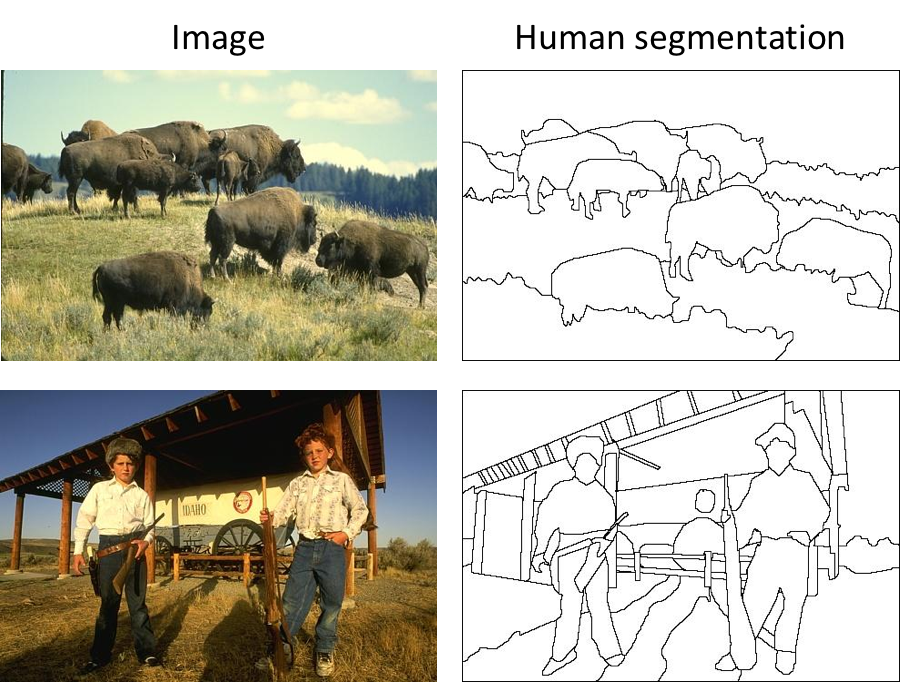
\includegraphics[width=8cm]{objects.png} \\
Figure 19:  Svetlana Lazebnik
\end{center}

We might also want to segment an image into many groups based off nearby pixels being similar. We call these groups "superpixels." Superpixels allow up to treat many individual pixels as one, and therefore allows us to perform some computations faster. Here is an example of an image segmented by superpixels:

\begin{center}
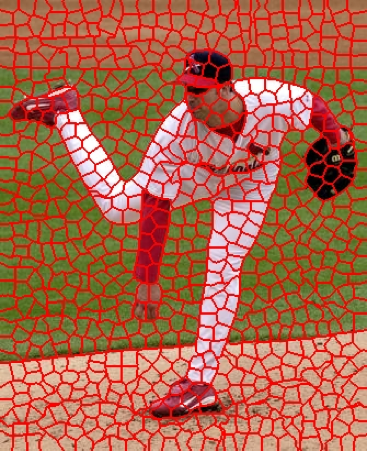
\includegraphics[width=8cm]{superpixels.png} \\
Figure 20: X. Ren and J. Malik. Learning a classification model for segmentation. ICCV 2003.
\end{center}

Superpixel segmentation and other forms of segmentation can help in feature support. We can treat the groups of pixels as one feature and garner information about the image from them. 

Segmentation is also beneficial for some common photo effects, such as background removal. If we can properly segment the image, we will be able to only keep the groups we want and remove the other groups.

While segmentation is clearly useful and has many applications, there is no one way to segment an image and we must compare different segmentation algorithms to find our optimal solution. If we run our segmentation algorithm and it comes back with very few groups that are too general, we have under segmented the image. If there are so many groups that the segmentation is no longer useful, then we have over segmented. However, even a properly segmented photo can have multiple different possible groupings.

To tackle the problem of how to segment an image, we will think of segmentation as clustering. By clustering, we are able to group similar data points together and represent them with one singular value. This again aids in our ability to manipulate the image or extract features from it. However, we must decide a few important issues:
\begin{enumerate}
\item How do we determine if two pixels, patches, or images are similar?
\item How do we compute an overall grouping from	
pairwise similarities?
\end{enumerate}
Different clustering algorithms answer these questions differently, and those algorithms will be discussed in depth in the next notes.

In general, the two broad categories of clustering algorithms are top down and bottom up. Top down clustering groups pixels and patches together because they lie on the same visual entity. Bottom up clustering groups pixels together because they are locally coherent.

We may also use certain visual patterns which humans recognize for our clustering algorithm. Some example patterns would be grouping similar objects together or using symmetry to aid in segmentation. In some instances, we can also look at "common fate." Common fate means that a group of objects appear to be moving together, so they share the same "fate." Here is an example of camels, which we can group by their common fate. 

\begin{center}
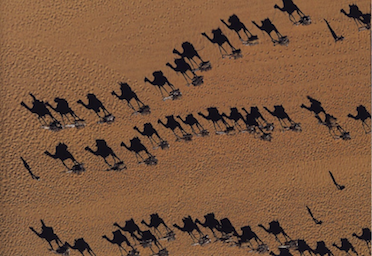
\includegraphics[width=8cm]{camels.png} \\
Figure 21: Arthus-Bertrand (via F. Durand)
\end{center}

We can also illustrate common fate with this optical illusion. This illusion, called the Müller-Lyer illusion, tricks us into thinking the bottom line segment is longer than the top line segment, even though they are actually the same length (disregarding the four mini-tails). 

\begin{center}
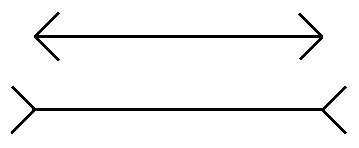
\includegraphics[width=8cm]{muller.jpg} \\
Figure 22: Simon Barthelme
\end{center}

Another way we can group objects is by proximity. With proximity, we group objects with what they appear to be close to. For instance, in this image, we might group the three people in the foreground together.
\begin{center}
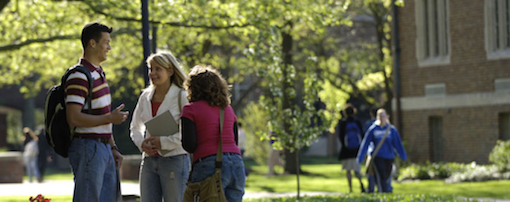
\includegraphics[width=8cm]{people.png} \\
Figure 23: Kristen Grauman
\end{center}


% References
\small
\bibliographystyle{plain}
\bibliography{bibliography}
\end{document}